\documentclass[a4paper,12pt]{article}
\usepackage[noabs,notoc]{HaotianReport}

\title{图片HSL空间色彩分析}
\author{刘昊天}
\authorinfo{电博181班, 2018310648}
\runninghead{数据可视化课程第一次作业}
\studytime{2019年04月}

\begin{document}
    \maketitle
    %\newpage
    \part{简答题回答}
    \section{小提琴图相关问答}
    \begin{figure}
      \centering
      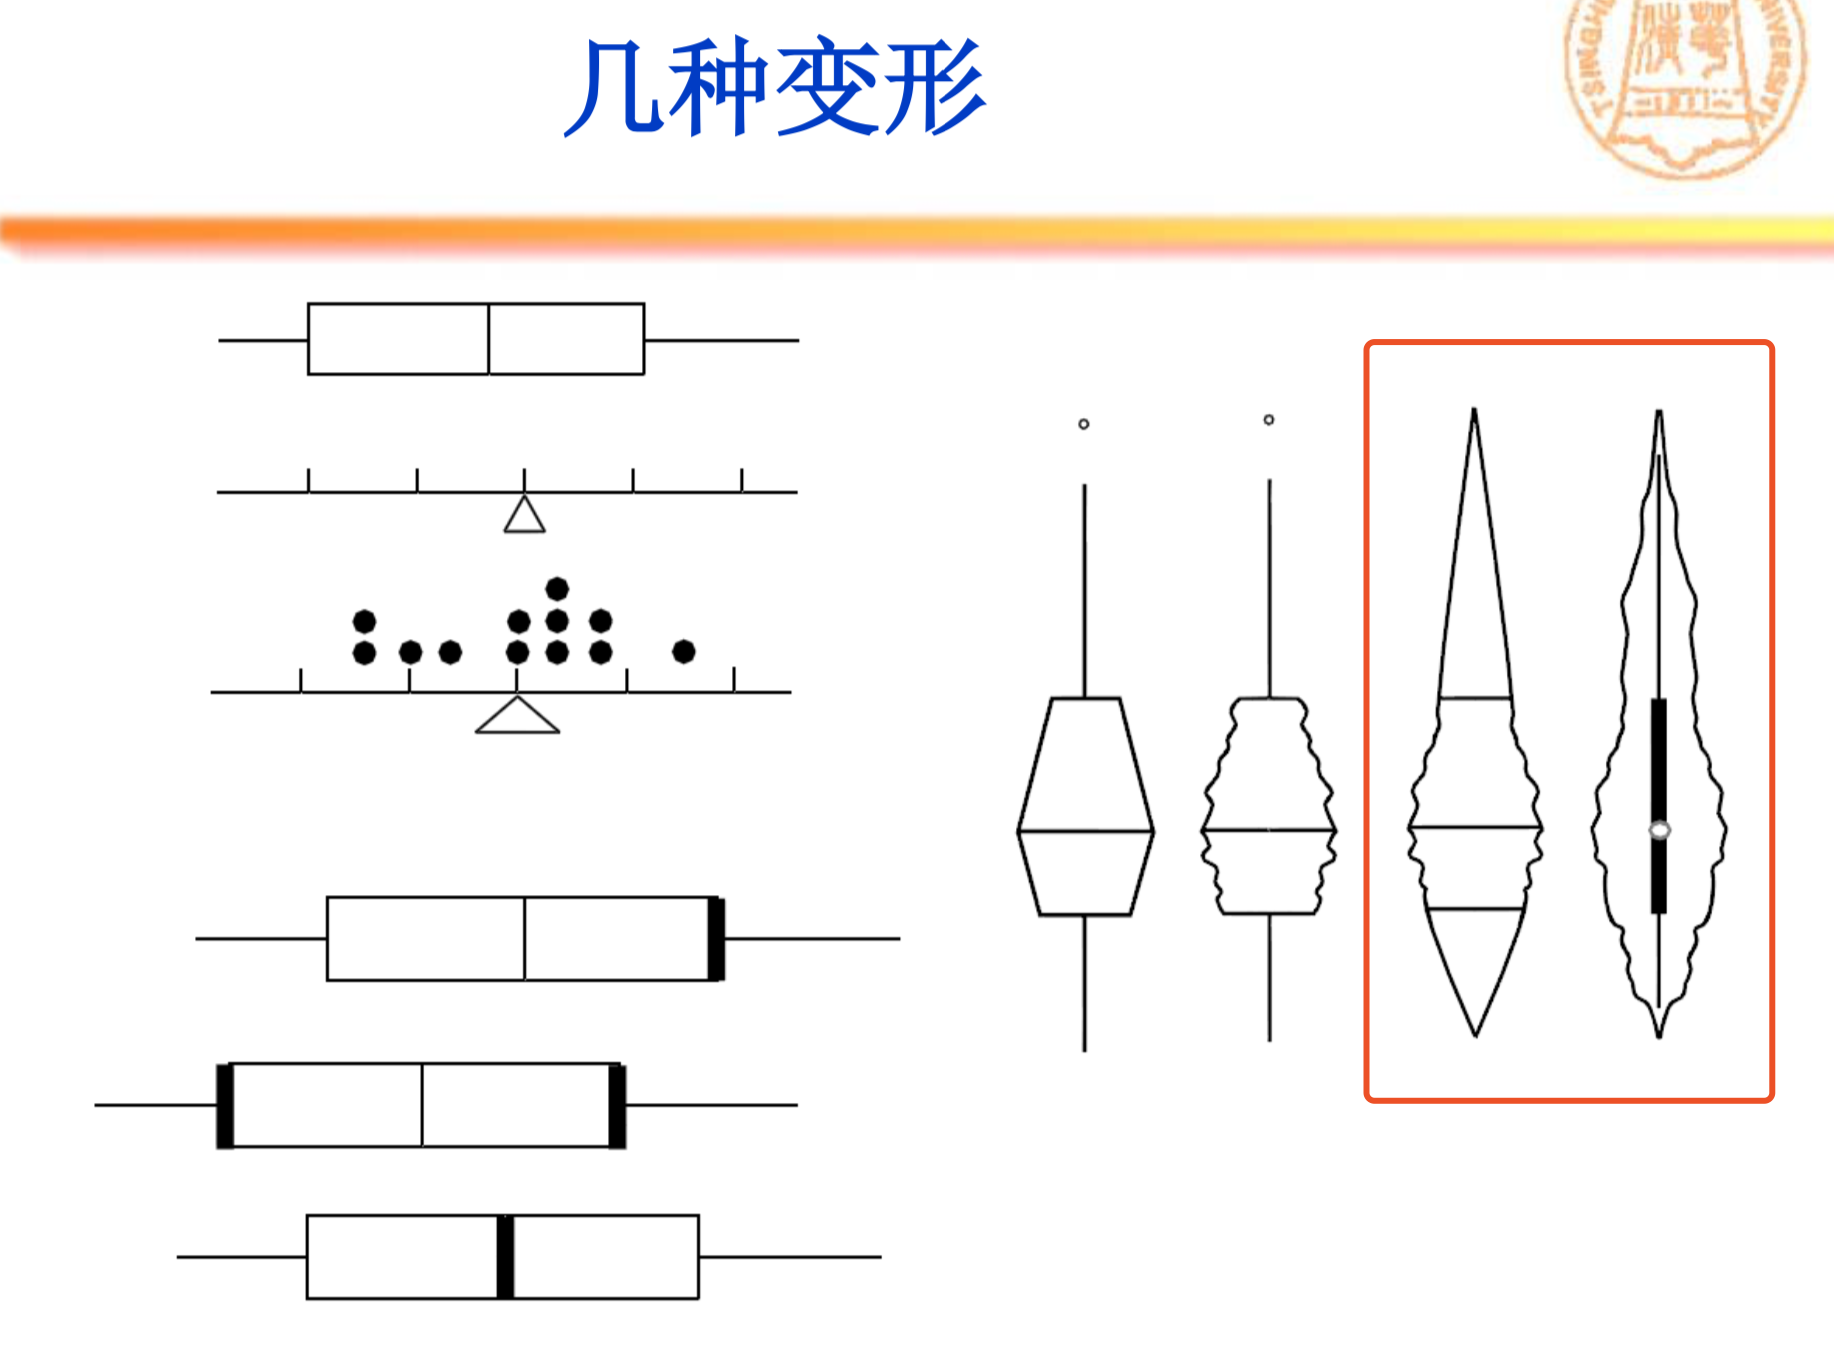
\includegraphics[width=0.8\linewidth]{ktviolin}
      \caption{课堂上出现的小提琴图}
      \label{fig:ktviolin}
    \end{figure}
    在第四讲第101页右侧,出现了小提琴图及变种,如\cref{fig:ktviolin}所示。

    小提琴图主要用于显示数据分布及分布的概率密度,因此适用于对比某指标不同值下另一指标分布情况的场景。例如,全国各省份居民年龄的分布情况,就可以用小提琴图展示;不同类型的群聊,用户收入的分布情况,也很适合用小提琴图展示。

    作为箱须图的变体图表,小提琴图可以展示有关数据分布的更多信息,而箱须图仅能展示大致的分布范围,而对分布本身没有细致刻画。

    也就是说,小提琴图包含了更多的细节,这也是其缺点所在。由于细节较多,可能会包含误导信息,反而无法观测到主要的分布情况。
    \section{圆环设计相关问答}
    更倾向于空心圆环,理由如下。
    \begin{enumerate}
      \item 空心圆环有展示原图的空间,在中心显示原图,可以更直观地呈现图片色彩的情况;
      \item 即便不展示原图,空心圆环使得色彩(信息)从圆心处的拥挤解放出来,能更清晰地展示;
      \item 最重要的是,类似于课堂上讲授的南丁格尔图表,圆形图表存在共有问题:采用角度编码,当离圆心越远时,呈现出的弧长越大,面积也越大,将使得外侧的区域更有优势。这在本例中,会使得大小比例发生变化,产生信息失真。如果不采用空心圆环,则圆心附近的小提琴图根本无法呈现;空心圆环一定程度上缓解了圆形图表带来的畸变问题。
    \end{enumerate}
    \part{编程题目说明}
    \section{概述}
    本程序主体是基于D3.js(或称D3)开发的。选择D3,一方面是由于JavaScript广泛应用于前端设计,在"轻量时代"更适合开发移动编写的应用程序;另一方面则是考虑到后续各问的可视化任务高度定制化,故应采用较为底层的绘制工具。D3全称是Data-Driven Document,即"数据驱动的文档",是一个用于数据可视化的JavaScript程序包,采用BSD-3开源协议托管于Github上。很多著名的JavaScript可视化工具,都是基于D3开发的。

    另外,本程序将各个可视化任务打包,统一在Web前端进行呈现,称为Colorana(意味Color Analysis),实现图片在HSL空间上的色彩分析。这部分采用了React.js+Material-ui的技术路线,二者均为开源程序。

    作业的成果Colorana托管在Netlify平台,地址为\url{https://color.nogeek.top}。由于前端的设计并非重点,因此该网站仅保证对Chrome的支持,且未对移动端进行针对性适配。本程序将在学期结束后以MIT协议开源。

    前端呈现如\cref{fig:frontend}所示,其中左上的选项卡可选择可视化项目,右下的控制区可控制绘制行为,右上展现了当前分析的图片。本报告中的样例图片即如图中所示。
    \begin{figure}[htbp]
      \centering
      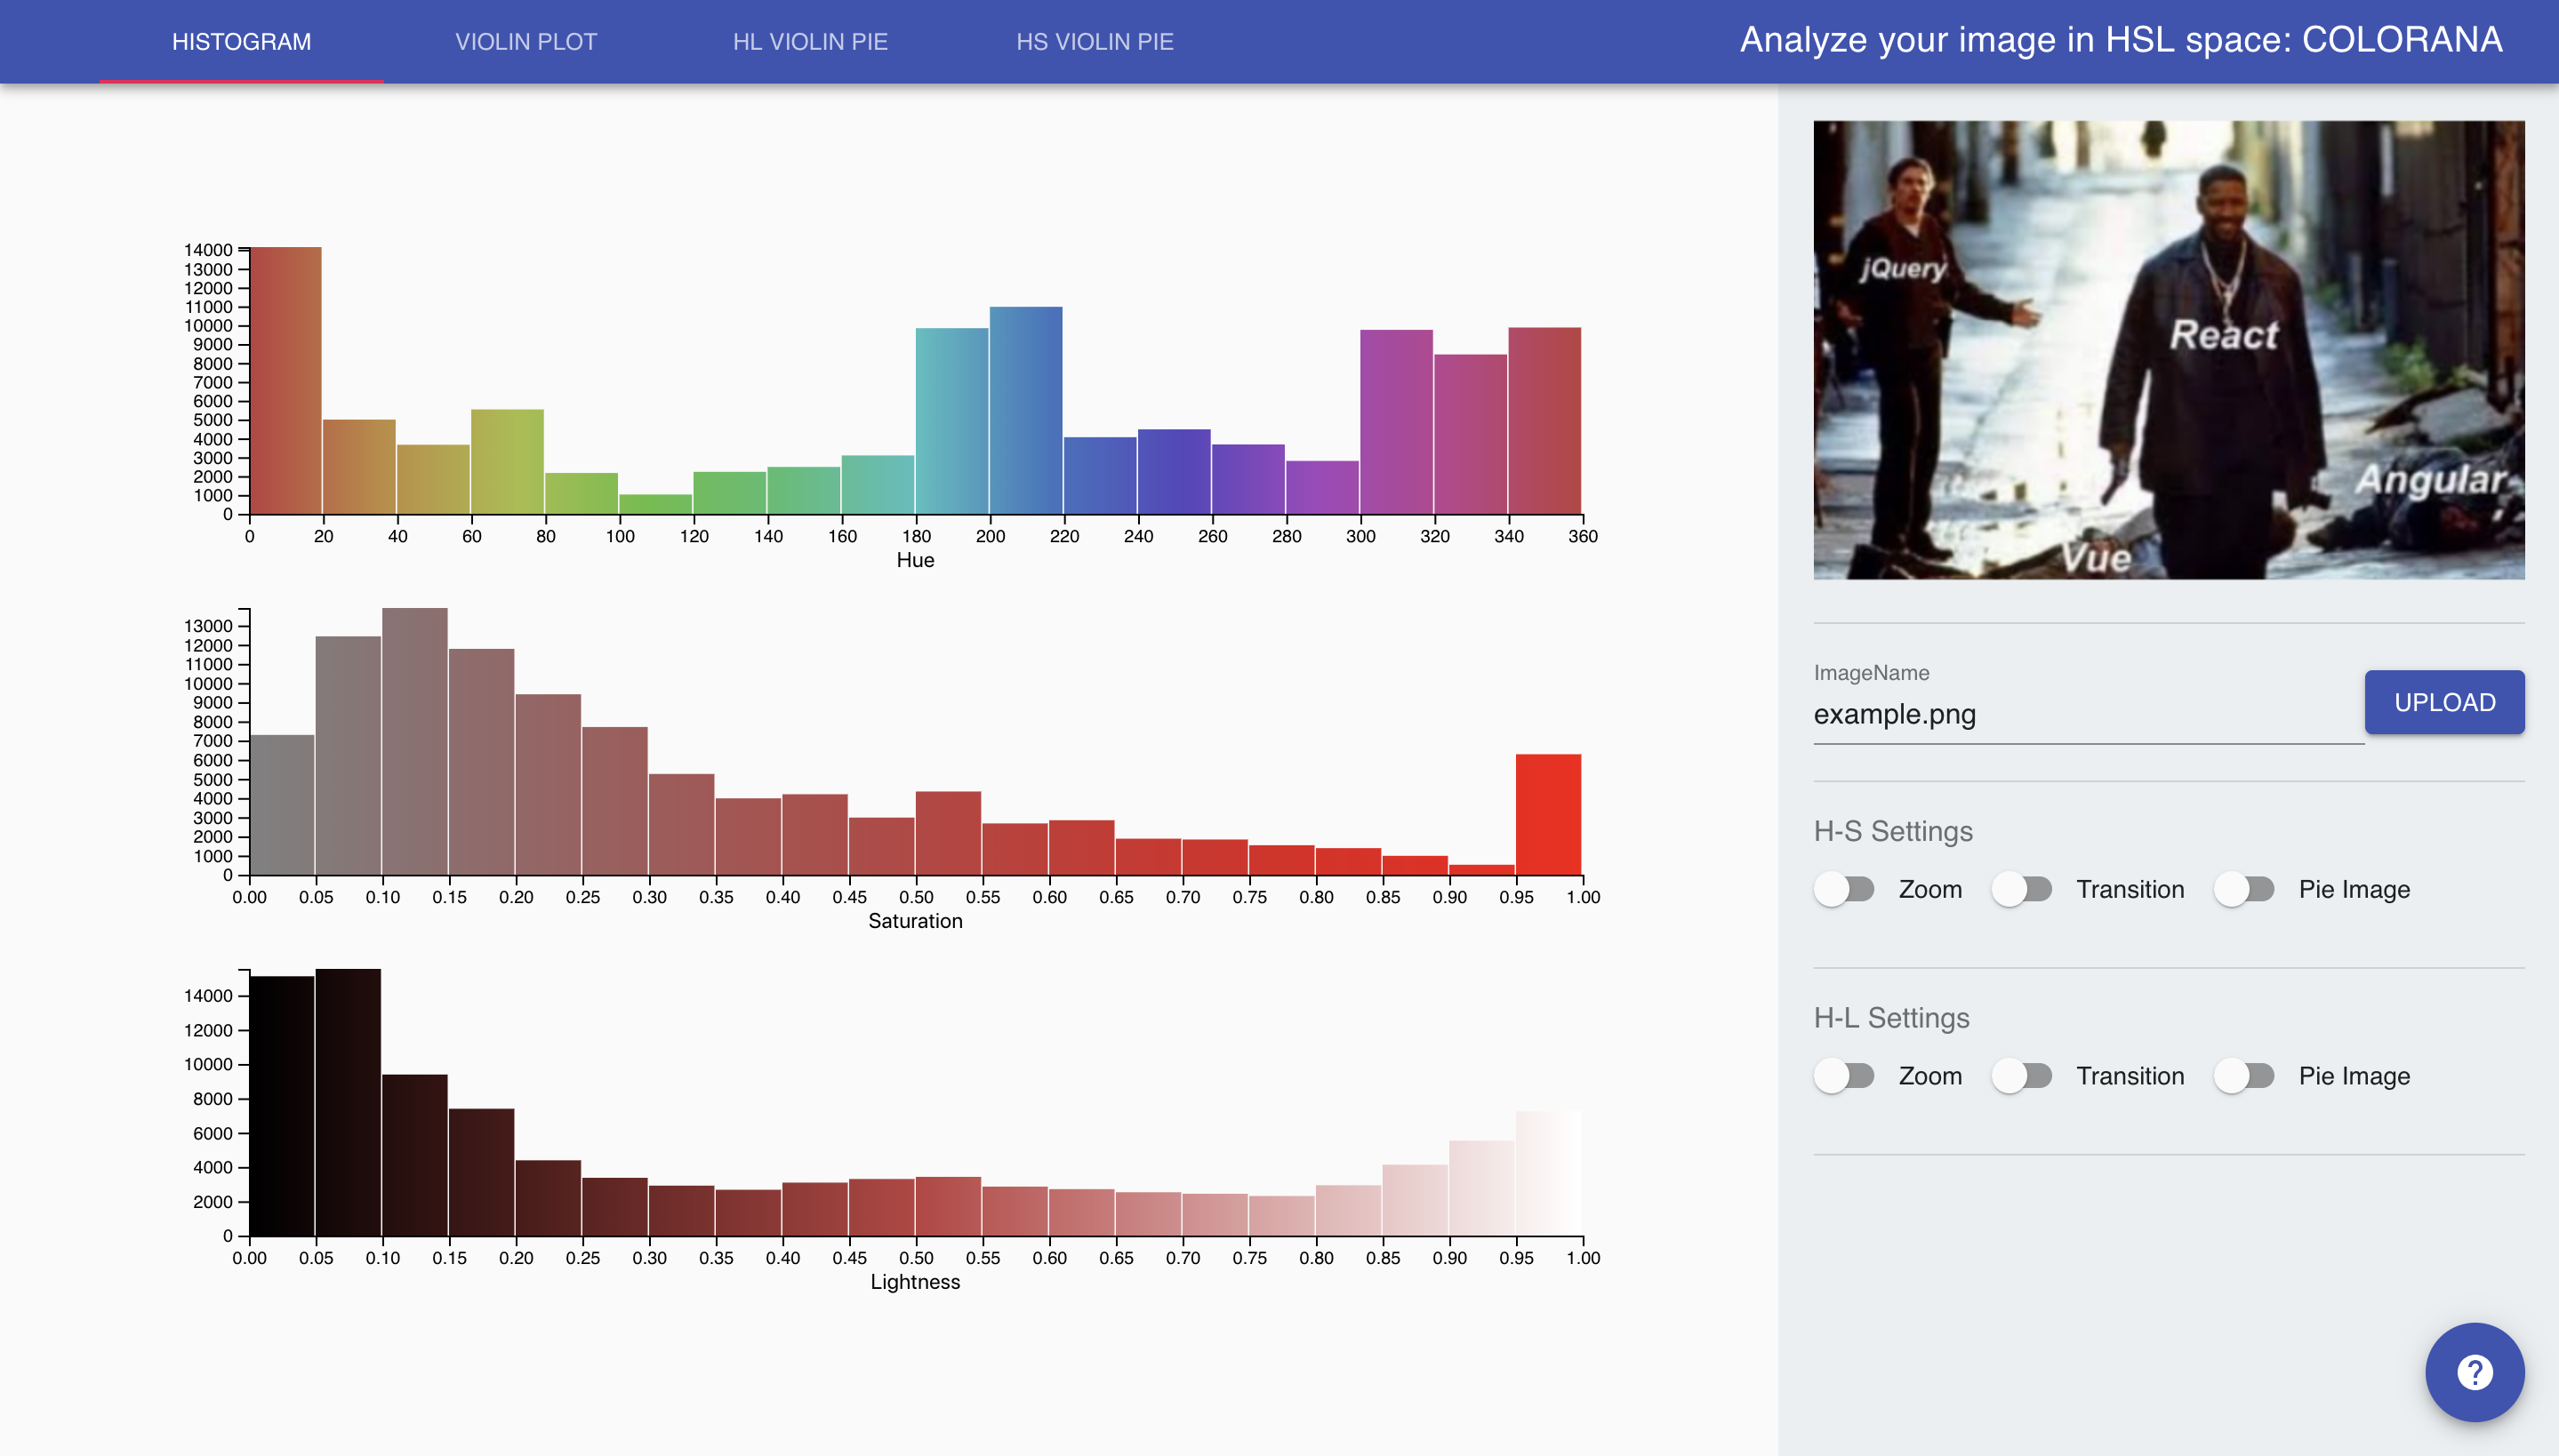
\includegraphics[width=0.9\linewidth]{frontend}
      \caption{程序前端呈现}
      \label{fig:frontend}
    \end{figure}
    \section{直方图绘制}
    \begin{figure}[htbp]
      \centering
      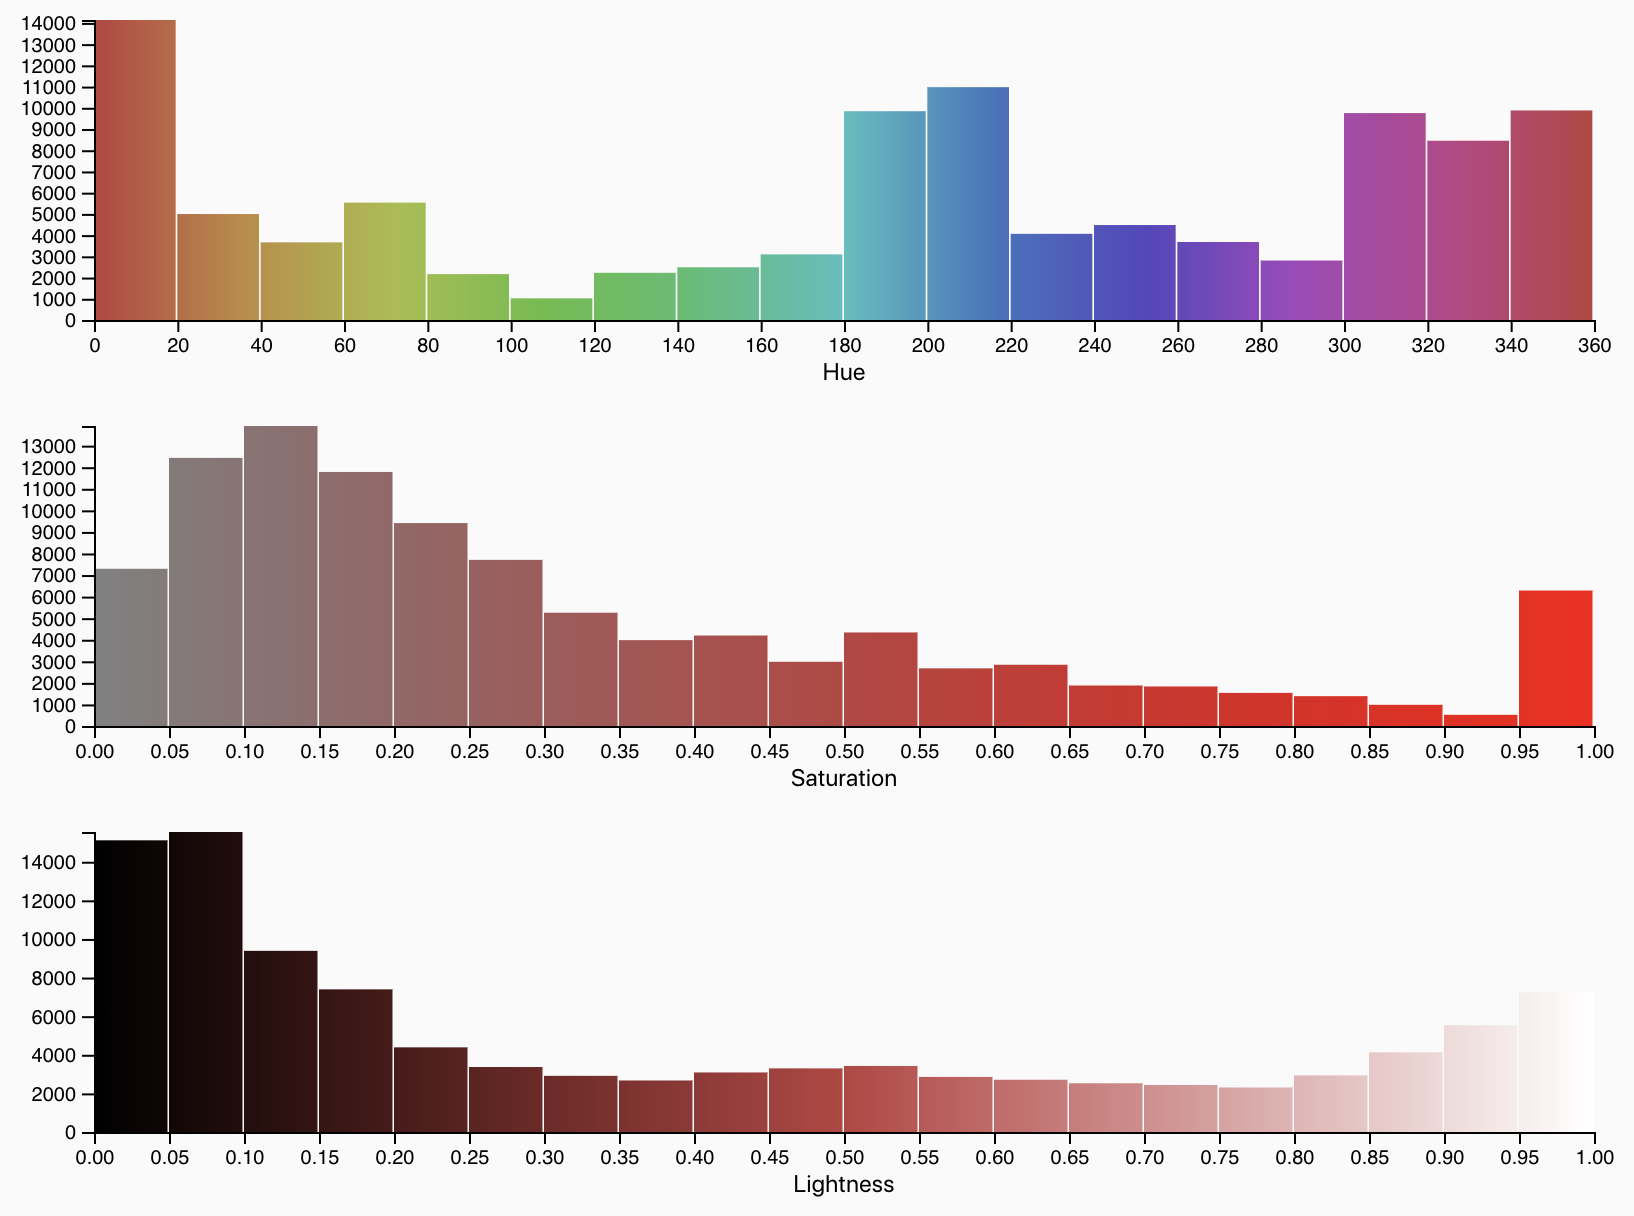
\includegraphics[width=0.9\linewidth]{histogram}
      \caption{HSL直方图}
      \label{fig:histogram}
    \end{figure}
    在\cref{fig:histogram}中实现了对HSL三个通道的直方图绘制,并在横向按照坐标用渐变颜色填充(当某通道不为自变量时,选取典型值为[h=0, s=0.5, l=0.5]),从而获得更直观的视觉效果。

    \paragraph{难点1} SVG中并不能定义HSL空间的插值函数,只能在RGBA空间实现渐变效果。该问题在其他各任务中同样存在。
    \paragraph{解决方案1} 在SVG中设置多个RGB插值点(实际为10个),依次按比例在HSL空间进行渐变,从而模拟HSL空间的色彩渐变效果。
    \section{小提琴图绘制}
    \begin{figure}[htbp]
      \centering
      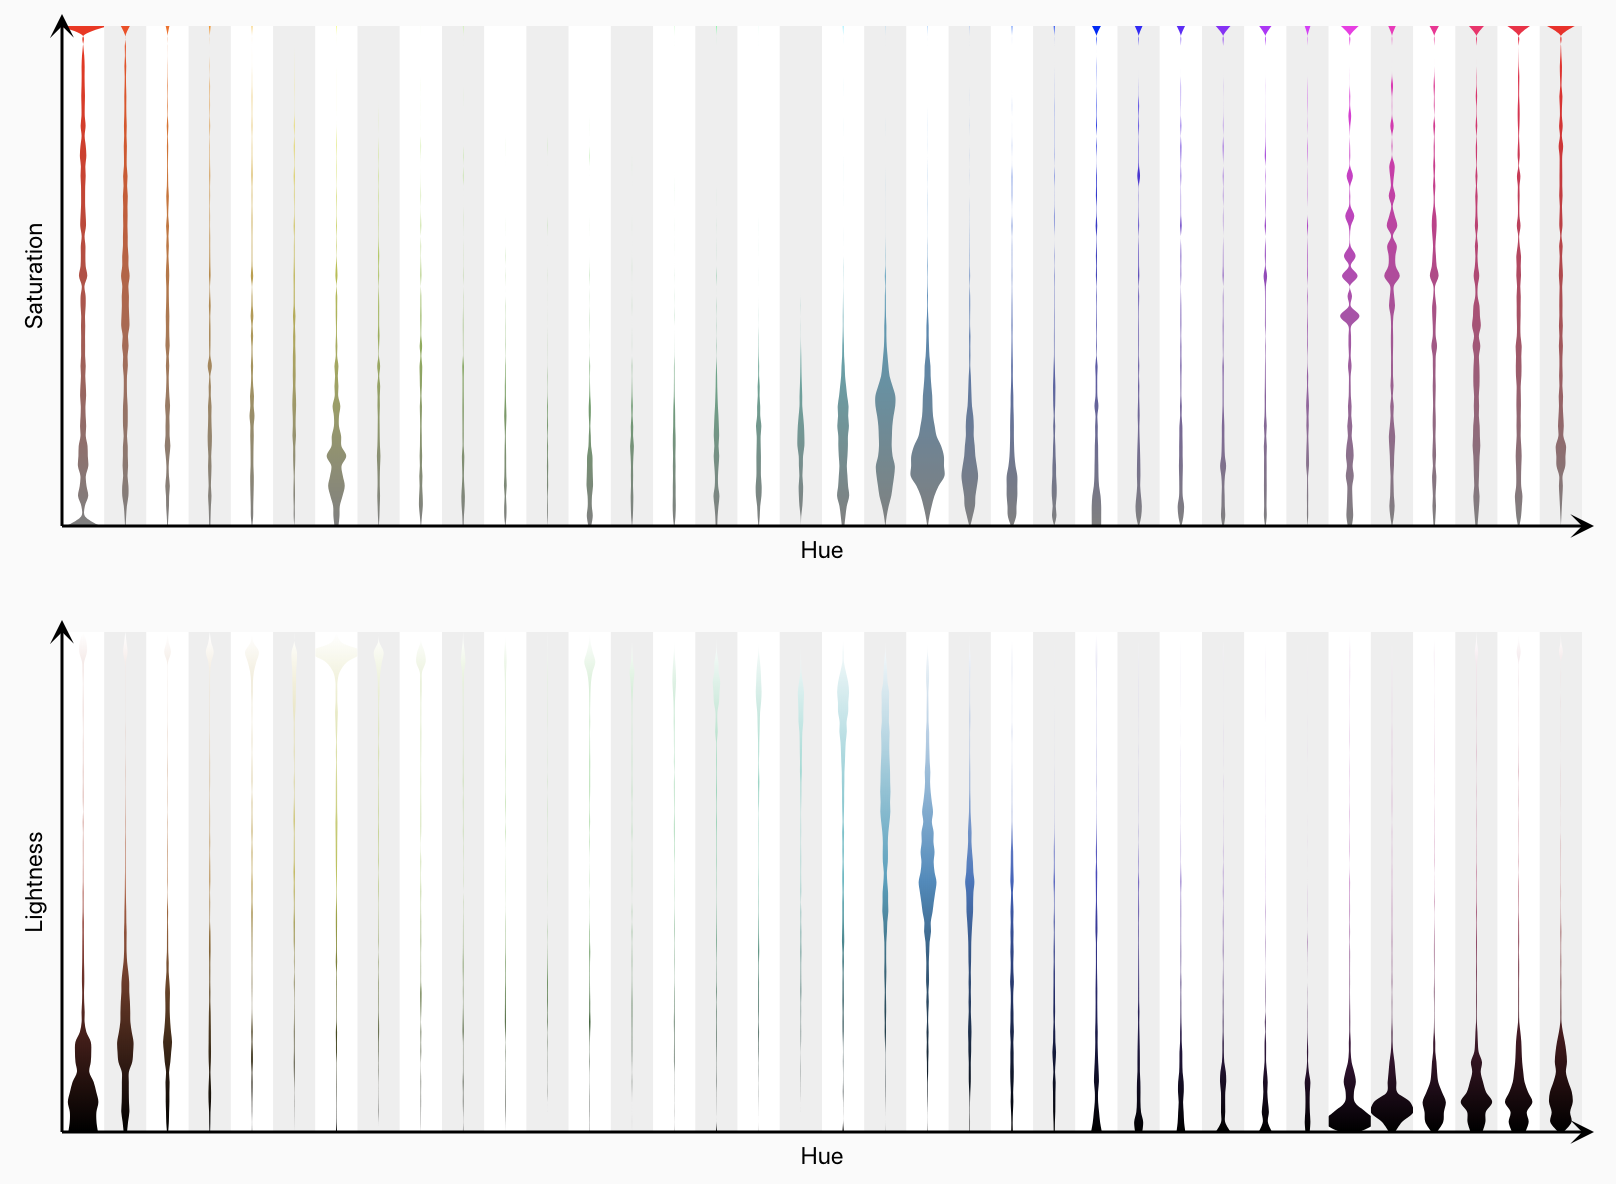
\includegraphics[width=0.9\linewidth]{violin}
      \caption{HSL小提琴图}
      \label{fig:violin}
    \end{figure}

    在\cref{fig:violin}中实现了对H-S及H-L的小提琴图绘制。可见,由于原图色彩偏暗,大部分色调的亮度都偏低,只有蓝色调亮度偏高,体现为原图中的远方石板路。同时蓝色调的饱和度偏低,而红色调饱和度偏高,体现为近处被夕阳照射的皮肤。

    \paragraph{难点2} 小提琴图排列紧密,相邻小提琴可能产生重叠。
    \paragraph{解决方案2} 在SVG中设置对每个色调分区建立<clippath>,并绑定到小提琴的<area>上。这个<clippath>的形状同坐标背景相间的栅格一致。

    \paragraph{难点3} 为保证大小关系,同一张图上每个小提琴绘制时的参考最大值为全局最大值,因此小提琴的"尾巴"可能太细,部分小提琴可能很难看清。
    \paragraph{解决方案3} 由于已经实现了clippath,我们可以有意识地让最大的小提琴溢出一部分,这样的溢出尽管损失了具体的大小信息,但"截断"的样式更能给人视觉冲击,同时还使得较小的部分显示清楚。
    \section{径向小提琴图绘制}
    \begin{figure}[htbp]
      \centering
      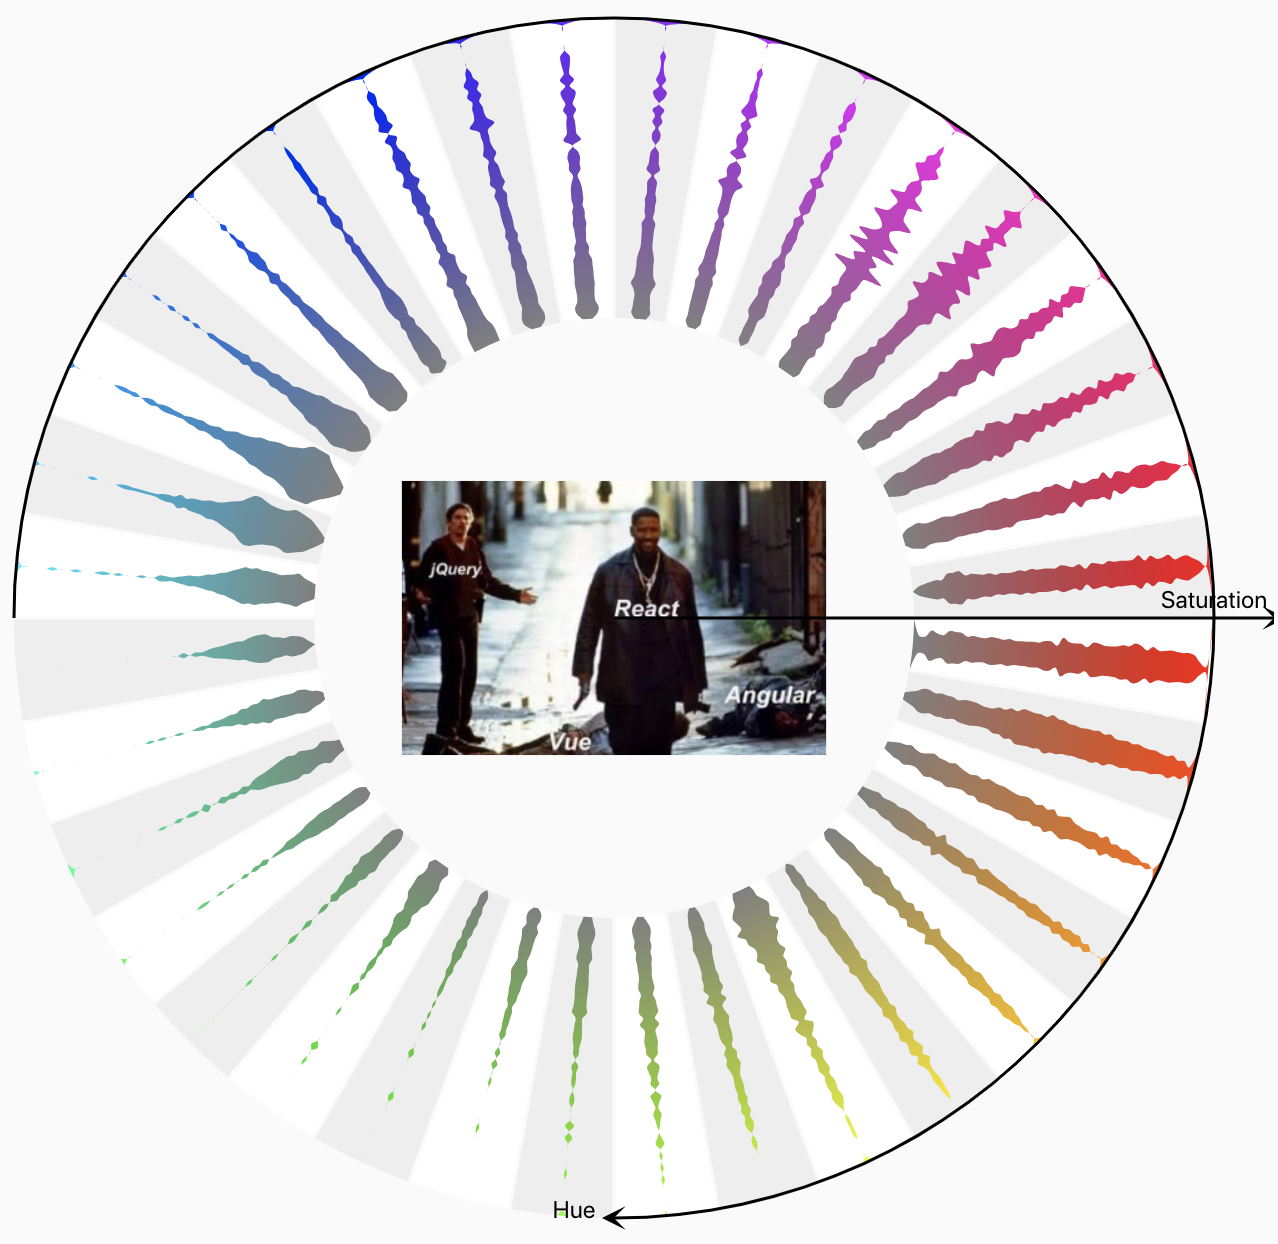
\includegraphics[width=0.5\linewidth]{hspie}
      \caption{H-S径向小提琴图}
      \label{fig:hspie}
    \end{figure}
    \begin{figure}[htbp]
      \centering
      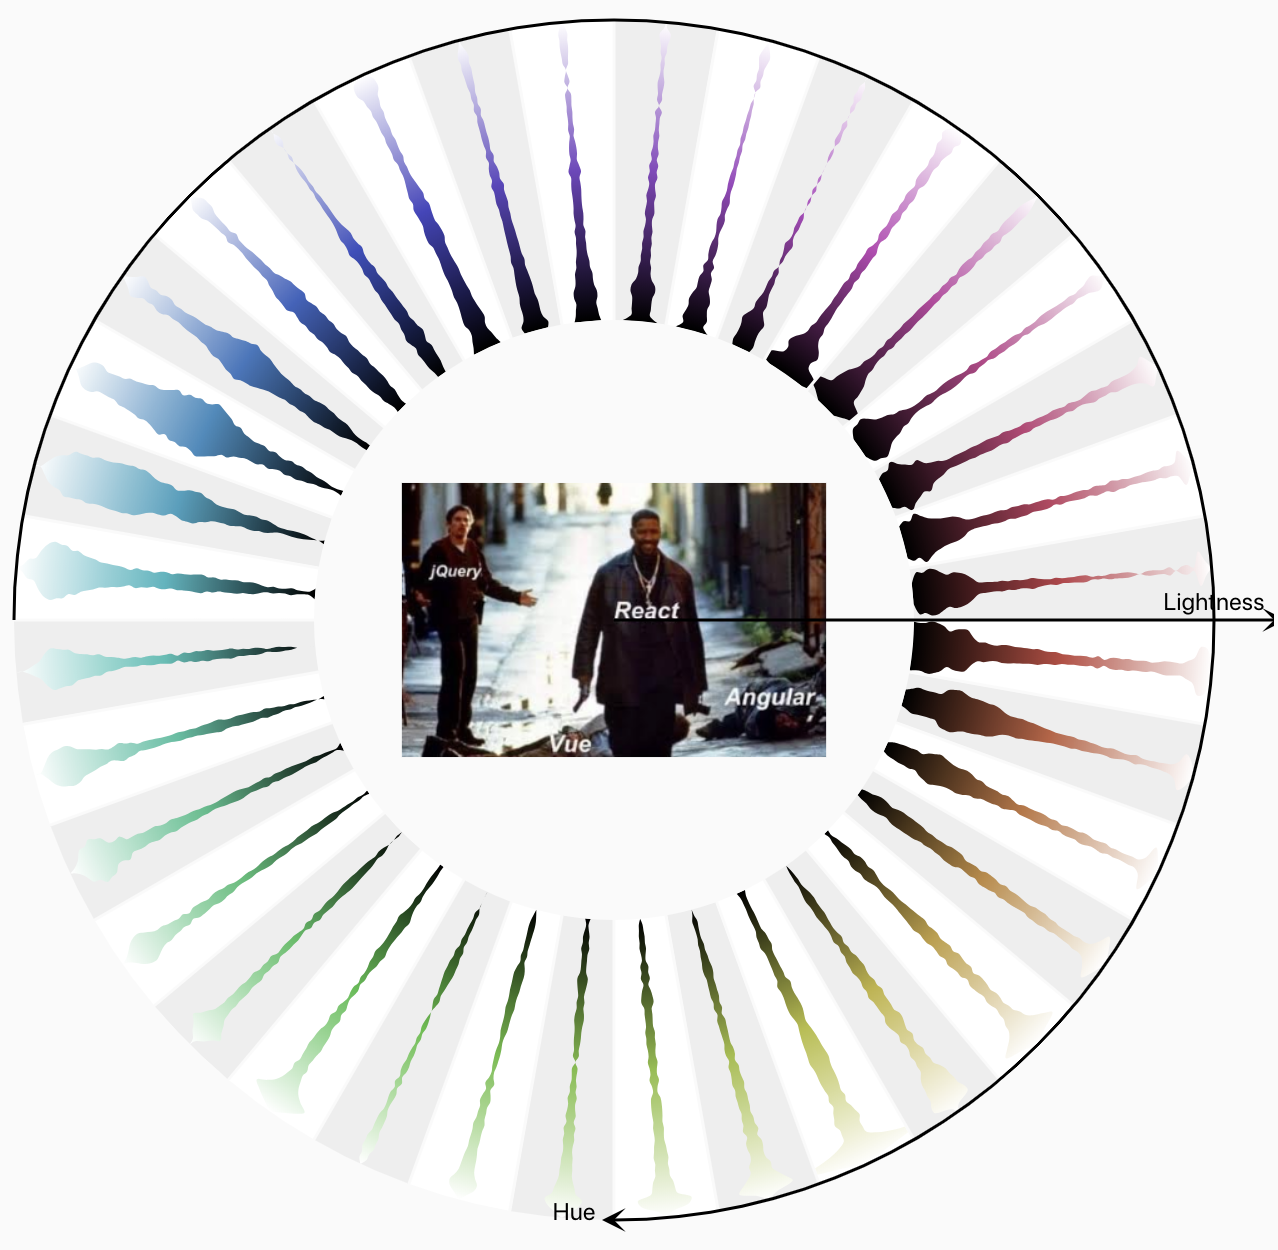
\includegraphics[width=0.5\linewidth]{hlpie}
      \caption{H-L径向小提琴图}
      \label{fig:hlpie}
    \end{figure}

    在\cref{fig:hspie,fig:hlpie}中分别实现了H-S通道和H-L通道的径向小提琴图绘制。在径向小提琴图中,我们展示的数据经过了一定的变换,从而增加了填充面积。

    \paragraph{难点4} 即便经过解决方案3的处理,空白区域依然过大。
    \paragraph{解决方案4} 对于小提琴图来说,必须保留的是各部分之间的大小关系。但是,具体的值大小未必需要精确,只要给用户的直观感受不变即可。因此,我们采用非线性函数变换的形式,降低最小值和最大值之间的对比,增大区域面积。此处选取的非线性函数为平方根函数。另外,作业例图在着色时似乎进行了截断,仅保留了较高亮度和饱和度的色彩。这种做法会使得数据的对应出现问题,传达的色彩信息将严重失真,本程序并未效仿。

    \paragraph{难点5} 扇形<clippath>绑定困难。SVG的clip逻辑是在transform前进行绑定,而为了方便绘制,小提琴图都是先绘制后transform:rotate()的,这样就不能正确绑定并遮罩。
    \paragraph{解决方案5} 将<clippath>反变换。
    \section{动画小提琴图绘制}
    \begin{figure}[htbp]
      \centering
      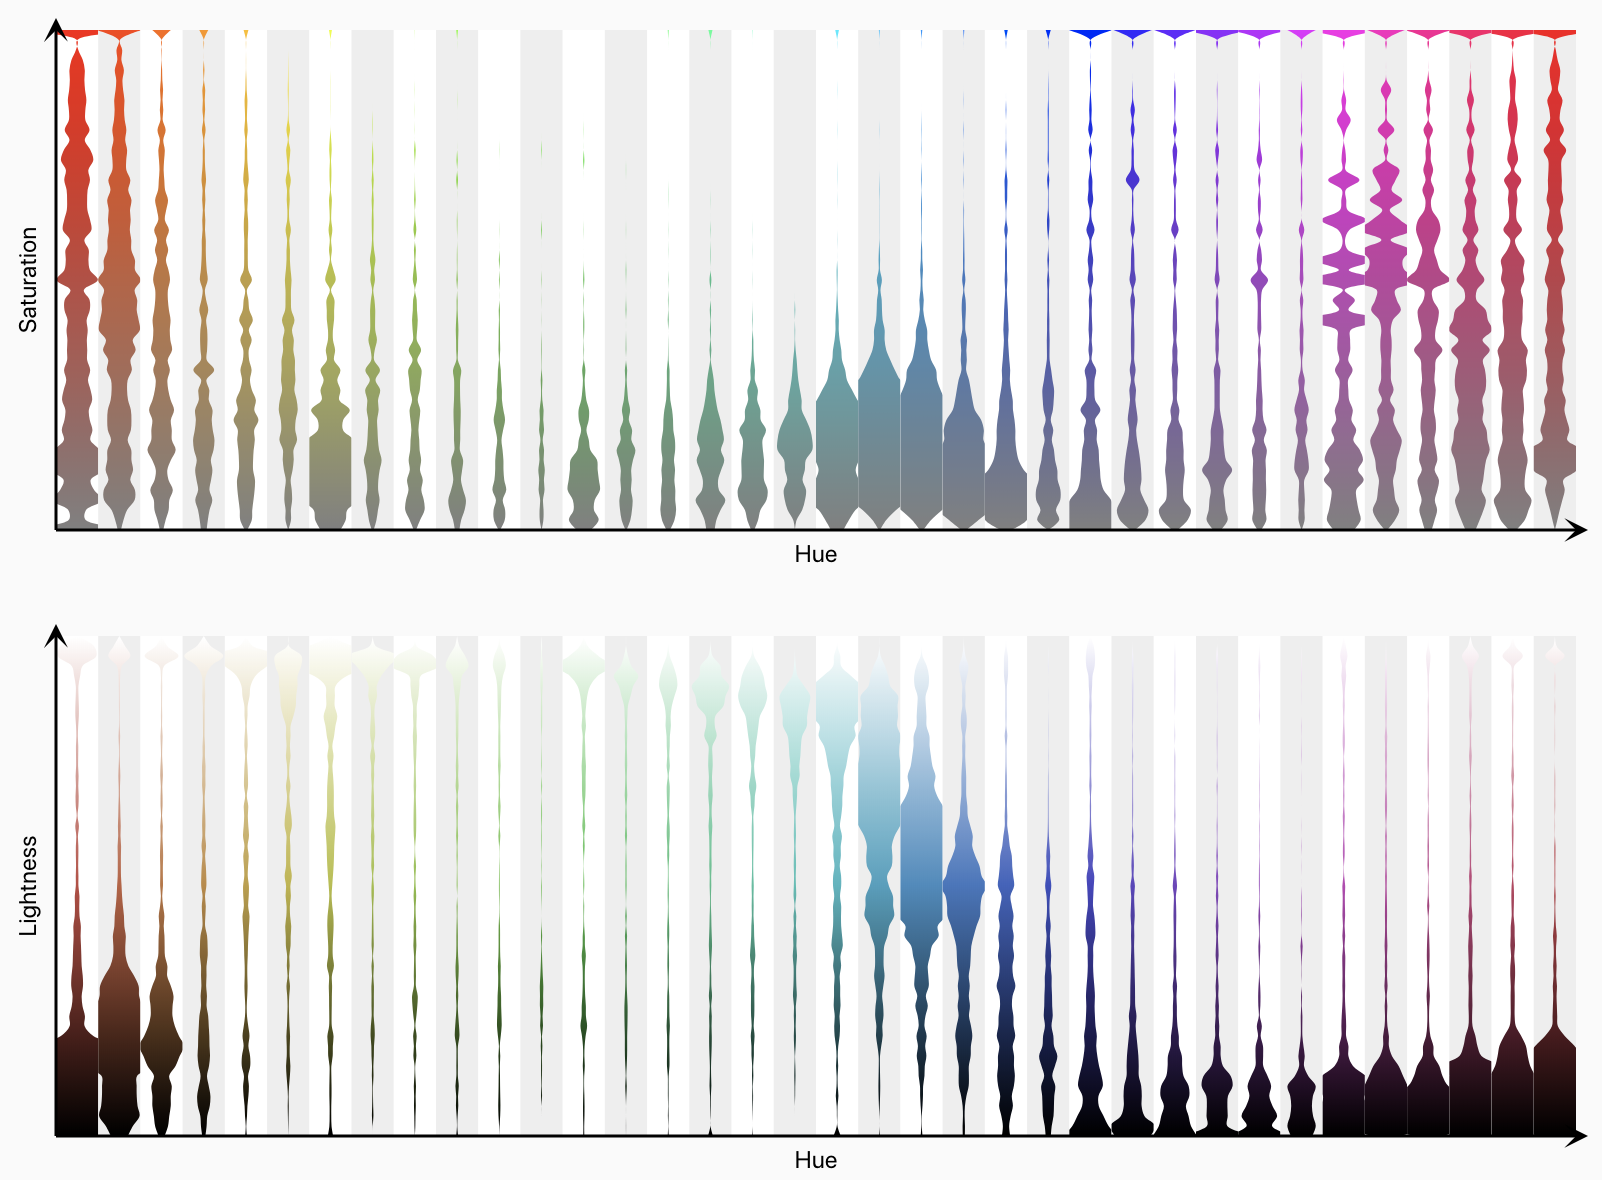
\includegraphics[width=0.9\linewidth]{trans}
      \caption{动画小提琴图}
      \label{fig:trans}
    \end{figure}

    \cref{fig:trans}展示了动画结束时的小提琴图,各小提琴在\cref{fig:violin}的基础上分别扩大了5倍宽度。由于pdf难以呈现动图,请访问\url{https://color.nogeek.top},并在右下角分别开启Zoom开关,并切换到"VIOLIN PLOT"选项卡,即可观看动图。

    这种呈现的效果要优于采用非线性变换的径向小提琴图,因为并未有信息失真,同时扩大后的图像更能让人了解图片的色彩分布。

    在\url{https://color.nogeek.top}中,还实现了多种选项的排列组合(Zoom:是否非线性变换,Transition:是否开启动画,PieImage:是否在圆环中显示图片)。

    \label{applastpage}
    \newpage
    \appendix
    \section{参考说明}
    \begin{enumerate}
      \item D3入门参考:精通D3.j3(第2版),吕之华. 电子工业出版社,北京,2017年。
      \item D3入门参考:D3官方文档,\url{https://github.com/d3/d3/blob/master/API.md}。
      \item 程序依赖:见package.json。
      \item React相关参考:开源项目ballot,\url{https://github.com/b1f6c1c4/ballot}。
    \end{enumerate}
\iffalse
\begin{itemize}[noitemsep,topsep=0pt]
%no white space
\end{itemize}
\begin{enumerate}[label=\Roman{*}.,noitemsep,topsep=0pt]
%use upper case roman
\end{enumerate}
\begin{multicols}{2}
%two columns
\end{multicols}
\fi
\end{document}
